
%%%%%%%%%%%%%%%%%%%%%%%%%%%%%%%%%%%%%%%%%%%%%%%%%%%%%%%%%%%%%%%%%%%%%%%%%%%%%%%%%%%%%%%%%%%%%%%%%%%%
\section{Susceptibility calculations}
    \label{Sec:3:SubsceptibilityCalculation}


To verify that we do get enhanced susceptibility, leading to a spin-density wave state, the $q$-dependant susceptibility -- described in section \ref{Sec:1:NestingSusceptibility} -- was calculated. Since the Lindhard function takes the sum over all energies in the Brillouin zone, there may be some concern that the rather crude adjustments to the DFT calculations performed in the previous section -- which have only been verified to be correct for energies at the Fermi surface -- may give erroneous results. However the nature of the Lindhard function means that far greater weight is given to energies that are near the Fermi surface and so, assuming that the energy dispersion does varies smoothly close to the Fermi level, it is unlikely to cause problems.

\begin{figure}[h!]
    \begin{center}
        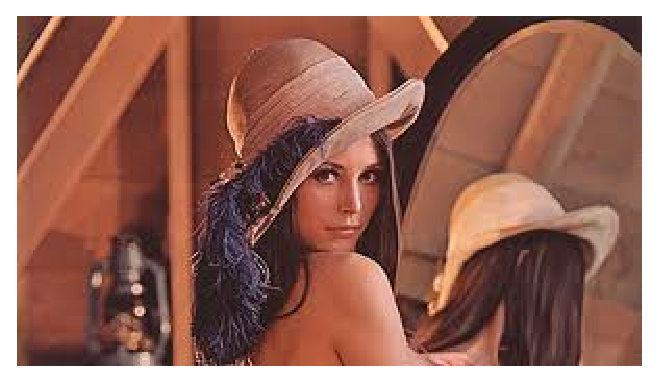
\includegraphics[scale=0.9]{Misc/TODO}
        \caption{The real part of the Lindhard susceptibility calculations for a free electron model with Fermi energy arbitrarily set to 5. Left panel shows the 2 dimensional calculation, the right shows the 3 dimensional calculation summed over all $k_z$}
        \label{Fig:3:FreeElectronSusceptibility}
    \end{center}
\end{figure}

Code to calculate the Lindhard susceptibility was written in MATLAB (Appendix \ref{Appendix:SusceptibilityCode} contains the full code) and early versions were tested with free electron cases in 2 and 3 dimensions with results shown in \ref{TODO}. This matches the expected free electron curves\footnote{See, for example, page 126 and Appendix F of reference\cite{Dressel2002}} and the code was adapted to accept output generated by WIEN2k. Further testing was performed by re-creating WIEN2k calculations on LaFeAsO$_{0.1}$F$_{0.9}$ performed by Mazin et al.\cite{Mazin2008} and then comparing our own susceptibility calculations using the new MATLAB code with the calculation in the Mazin paper. A temeprature smearing of \unit[1]{mRy} was quoted in the Mazin paper which was equated, using the Boltzman conversion, to a temperature of \unit[157.88]{K}. Results are presented in \fig\ref{Fig:3:MazinX0Comparison} and the agreement is evident.

\begin{figure}[h!]
    \begin{center}
        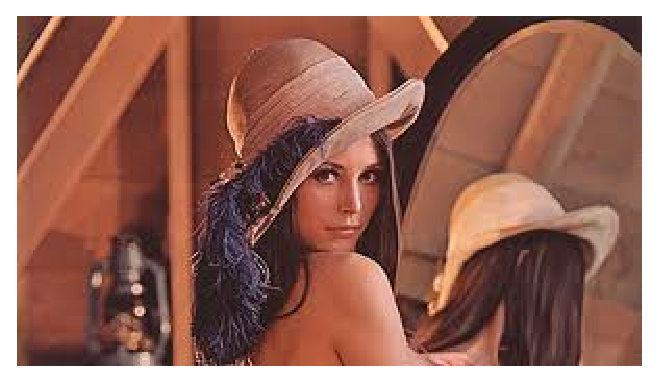
\includegraphics[scale=0.9]{Misc/TODO}
        \caption{Left hand panels show the real and imaginary parts of Lindhard susceptibility calculations on LaFeAsO$_{0.1}$F$_{0.9}$ by Mazin et al. summed over all $k_z$, right panels show the same calculation performed using our own MATLAB code.}
        \label{Fig:3:MazinX0Comparison}
    \end{center}
\end{figure}

\begin{figure}[h!]
    \begin{center}
        \includegraphics[scale=0.9]{Chapter3-dHvABaFe2P2/Figures/AngleDepMeasurements/SusceptibilityTempSmearing/SusceptibilityTempSmearing}
        \caption{The Fermi distribution plotted at various temperatures using a contrived free electron distribution of energies scaled to the results of band 1 DFT calculations. An arbitrary Fermi energy of \unit[0.6]{Ry} is shown. The vertical lines shown the distribution of points in the model and are to illustrate the amount of smearing over points in the model that occur.}
        \label{Fig:3:SusceptibilityTempSmearing}
    \end{center}
\end{figure}

Applying a temeprature smearing to the function is useful to gloss over the finite element size in the calculation which can cause significant spikes in the results. \Fig\ref{Fig:3:SusceptibilityTempSmearing} shows the smearing at particular temperatures. The choice of temperature depends on the granularity of your model as well as the expected fine detail of the results. For our calculations a temperature of \unit[158]{K} was used which corresponds to \unit[1]{mRy} which was the smearing used in a similar investigation into LaFeAsO using a comparable number of data points\cite{Mazin2008}.

Calculations were performed in MATLAB using a $93\times93\times93$ grid of energy values that covered the first Brillouin zone. A small $\delta$ of $10^{-6}$ was included in order to obtain the imaginary component of the susceptbility.

\begin{figure}[h!]
    \begin{center}
        \includegraphics[scale=0.9]{Chapter3-dHvABaFe2P2/Figures/AngleDepMeasurements/SusceptibilityEnhancement/SusceptibilityEnhancement}
        \caption{Left panel shows the maximum $q$ dependant susceptibility in each plane perpendicular to $q_z$ between bands $1$ and $4$. Results where calculated with \unit[1]{mRy} of temperature smearing and $\delta=1\times10^{-6}$. Right panel shows the susceptibility in the plane at $q_z=1.5$ which is typical of all the $q_z$ planes for this band combination.}
        \label{Fig:3:SusceptbilityEnhancement}
    \end{center}
\end{figure}

\Fig\ref{Fig:3:FullSusceptibility} shows the total susceptibility coupling across various band combinations.

\begin{figure}[h!]
    \begin{center}
        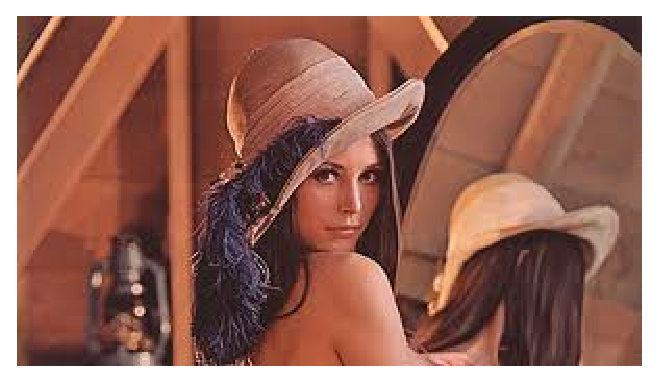
\includegraphics[scale=0.7]{Misc/TODO}
        \caption{}
        \label{Fig:3:FullSusceptibility}
    \end{center}
\end{figure}

